\documentclass[11pt]{article}
\usepackage[margin=1.1in]{geometry}
\usepackage{amsmath,amssymb}
\usepackage{booktabs}
\usepackage{graphicx}
\usepackage[hidelinks]{hyperref}
\usepackage{xcolor}
\usepackage{pgfplots}
\pgfplotsset{compat=1.17}
\usetikzlibrary{arrows.meta,positioning}
\definecolor{accent}{RGB}{42,101,175}
\definecolor{corrupt}{RGB}{201,109,44}
\definecolor{inkmut}{RGB}{110,118,126}

\title{Design by Falsification:\\
Distilling an Evidence-Bound Multi-Agent Harness from the\\
Registered Failures of a Council-of-Experts Pipeline}
\author{Sam Bobo}
\date{Draft v0.3, September 2026}

\newcommand{\ci}[2]{\ensuremath{[#1,\,#2]}}

\begin{document}
\maketitle

\begin{abstract}
Multi-agent pipelines that route a task through domain-specialist
language models and synthesize their contributions through a lead
writer rest on several premises: that specialists contribute knowledge
a generalist lacks, that instructions can make the writer epistemically
careful, and that a model can recognize when it is out of its depth.
This paper reports a falsification-first evaluation of such a
council-of-experts architecture across more than fifty pre-registered
experiments on auditable local hardware (7 to 20B parameter models), in
which nearly every premise failed its registered test. Specialist
fine-tunes carry per-model rather than per-domain signatures; an
epistemic instruction installs only its named phrase; preference judges
then penalize that phrase; stable model self-reports (confidence,
priors, ownership) do not predict behavior; and prose transports only
$0.11$ to $0.33$ of the epistemic qualification supplied to it. The
falsifications localize mechanisms, and the mechanisms compose into an
orchestration harness in which redundancy is engineered rather than
assumed, epistemic qualification travels outside the writer's prose,
re-consultation is triggered by mandated artifacts rather than
self-assessment, and no component is retained on rationale alone. Each
load-bearing design rule was then re-tested prospectively as its own
registered experiment. Assigning a contested quantity to a second
specialist halves corrupted-value adoption (from $0.900$ to $0.450$);
an appendix assembled outside the writer carries $100\%$ of specialist
caveats against the $17\%$ that survives prose, changes downstream
decisions ($+0.691$ over a matched irrelevant control) at parity with
in-prose placement, and shows no detected preference cost; and the full
re-consultation loop closes with a live specialist ($0.905$ adoption
versus $0.333$ control, within noise of a scripted ceiling). Two
registered tests contradicted the design rationale: sibling isolation
lost its contamination warrant to an informative null, and an elicited
ownership rule failed its confirmation experiment at exactly chance.
Both demotions are recorded in place. The paper argues that this
acquisition path, retaining only components that survive registered
attempts to falsify them, is the appropriate standard for multi-agent
architecture.
\end{abstract}

\section{Introduction}
\label{sec:intro}

The architecture under study follows a design that was conventional
in 2024 and 2025. Three domain-specialist models (healthcare, legal,
finance) each analyze a decision problem from their own expertise, and
a lead writer synthesizes their contributions. Aggregation pipelines of
this shape report state-of-the-art preference results
\cite{wang2024moa}; specialist fine-tunes are widely available; and the
architecture's premises appear almost too obvious to test. Specialists
contribute what generalists cannot. Instructing the lead to preserve
uncertainty makes it careful. A model that is out of its depth can say
so. Corroboration among specialists strengthens claims.

This paper reports what happens when those premises are tested. The
research program ran as a falsification-first ledger: every experiment
was pre-registered with predictions, falsification conditions, and
attainability computed from the archive before any run; every deviation
and verdict was recorded; and the instruments themselves were audited,
producing fourteen recorded instrument-validity findings. A companion
paper \cite{bobo2026audit} reports the audit findings in full. The
present paper makes the systems argument: it describes what remains of
a multi-agent architecture after most of its premises fail registered
tests, and what can be constructed from the parts that survive.

The argument proceeds in four stages.

\begin{enumerate}
\item \textbf{The premises failed} (Section~\ref{sec:premises}). They
failed registered experiments with pre-stated kill conditions, most of
which fired.
\item \textbf{The failures localized mechanisms}
(Section~\ref{sec:survivors}). Each falsification identified a real
mechanism: the lead is a source selector rather than a verifier;
instruction compliance is not behavior; and the scarce resource in
consultation is the trigger, never the capability.
\item \textbf{The mechanisms compose into a harness}
(Section~\ref{sec:harness}). If protection is coverage, coverage can be
engineered. If prose loses epistemic content, that content need not be
shipped in prose. If self-assessment is empty, triggers can be drawn
from mandated artifacts instead.
\item \textbf{The harness was then tested component by component}
(Section~\ref{sec:retests}). The load-bearing components survived with
causal or predictive effect sizes; one design rationale was demoted by
an informative null; one candidate rule was rejected by its own
confirmation experiment; one gate failed its frozen criteria twice and
is recorded as not deployable; the accuracy question was resolved as
untestable for lack of headroom; and the assembled bundle was compared
head-to-head against the original architecture and ships its machinery
at no detectable preference cost. The architecture that remains is
smaller than the one designed and better than the one assumed.
\end{enumerate}

\paragraph{Methodological claim.} Multi-agent frameworks commonly ship
components on rationale: a verification stage because verification
sounds prudent, a confidence threshold because calibration sounds
measurable, a debate round because deliberation sounds epistemic. The
central claim of this paper is that every component of a multi-agent
system is an empirical claim about model behavior, and that most such
claims are false at the scale where practitioners actually deploy them.
The harness presented here is not offered as the best possible
architecture. It is offered as the subset of one architecture that
survived more than fifty registered attempts on its premises, with the
verdicts, including the demotions, attached to the components they
license.

\paragraph{Contributions.} The paper makes the following contributions.
\begin{enumerate}
\item A ledger of nine architectural premises for specialist
aggregation pipelines, each with its registered test and verdict, in
which seven are falsified, one is null, and one is resolved as
untestable at the studied scale (Section~\ref{sec:premises}).
\item An orchestration harness in which each component is derived from
a specific verdict and does only what that verdict licenses
(Section~\ref{sec:harness}).
\item Prospective single-factor re-tests of each load-bearing harness
component, with effect sizes, confidence intervals, and two recorded
demotions of the design's own rationales (Section~\ref{sec:retests}).
\item A head-to-head comparison of the assembled harness against the
original architecture under a validated order-debiased two-family
preference protocol (Section~\ref{sec:retests}).
\item A statement of operating economics and open risks, each attached
to the component it concerns (Section~\ref{sec:economics}).
\end{enumerate}

\section{Related Work}
\label{sec:related}

\paragraph{Aggregation pipelines.} Mixture-of-Agents
\cite{wang2024moa} and its successors report preference gains from
aggregating multiple proposer outputs through an aggregator model.
Self-MoA \cite{li2025selfmoa} shows that mixing weaker models often
degrades results, a finding consistent with the per-model signature
result reported here. Debate and multi-agent discussion studies
\cite{wang2024rebuttal} find gains concentrated where prompts were
weak, consistent with the finding that the one intervention retained
here routes information rather than deliberation.

\paragraph{Judge pathologies.} Critiques of LLM-as-a-judge evaluation
\cite{zheng2023judging} motivate the order-debiased two-family
protocol used throughout. Length and sycophancy pressures under
preference optimization \cite{singhal2023length,sharma2023sycophancy}
sharpen into the measured phrase penalty reported in the companion
audit.

\paragraph{Pre-registration in systems research.} No prior work is
known to the author that pre-registers each component of a multi-agent
architecture and reports the failures alongside the survivals. That
practice, more than any single component, is what this paper proposes
for adoption.

\section{Background}
\label{sec:background}

\subsection{The council-of-experts pipeline}

The audited pipeline is a two-layer aggregation architecture. Three
specialist seats, each a prompted or domain-fine-tuned 7 to 8B model or
a role-prompted sample of the writer, receive a decision problem and
produce independent contributions. The contributions are concatenated
and passed to a 20B mixture-of-experts writer (\texttt{gpt-oss:20b})
operating as the lead, under either a published aggregate-and-synthesize
prompt or a minimal lead-analyst prompt. The case battery consists of
eighteen strategic advisory scenarios spanning healthcare, legal, and
finance content.

\subsection{Registration protocol}

Every experiment in the program is registered before it runs. A
registration states the hypotheses, the falsification conditions, the
attainability computation (the fraction of runs in which the outcome
variable can fire, computed from existing data for every registered
prediction), and the consequences of each verdict. Verdicts are entered
in a status ledger that distinguishes live, provisional, withdrawn, and
blocked claims. Three program-level audits re-classified earlier
results, and null results are cited only at the strength their audit
class permits (informative, weak, uninformative, or degenerate).
Registrations are committed to the repository before first runs, so
temporal ordering is verifiable from version history.

\subsection{Terminology}

The ledger refers to each registered experiment as a \emph{cell}; the
term is retained here where a specific ledger entry is cited (for
example, C55). A \emph{seat} is one specialist position in the
pipeline. The \emph{lead} is the synthesizing writer. The
\emph{orchestrator} is the non-model control layer that plans,
dispatches, and assembles. \emph{Transport} denotes the fraction of
epistemic qualification supplied upstream that appears in the lead's
output. Confidence intervals are cluster-bootstrap intervals over cases
unless stated otherwise.

\section{Premises That Failed Registered Tests}
\label{sec:premises}

Table~\ref{tab:premises} summarizes the program's negative results.
Each row lists a premise the council architecture requires, the
registered experiment that tested it, and the verdict. Effect sizes and
protocols are reported in the companion paper; here each premise is
given one sentence of mechanism.

\begin{table}[t]
\centering\small
\begin{tabular}{p{0.34\textwidth}p{0.24\textwidth}p{0.32\textwidth}}
\toprule
Premise required by the council & Test & Verdict \\
\midrule
Specialist fine-tunes share a domain signature & two medical tunes of
one base versus their base & \textbf{falsified}: signatures are
per-model; the tunes disagree with each other \\
An epistemic instruction changes the lead's behavior & counterbalanced
phrase-swap; synonym forms & \textbf{falsified}: the named phrase
appears ($0.67$ to $0.70$); the construct beyond it is unchanged
(CIs \ci{-0.079}{+0.111}, \ci{-0.103}{+0.087}) \\
Careful marking is at worst neutral under evaluation & order-debiased
preference, phrase arms versus own control & \textbf{reversed}: the
phrase \emph{loses} preference ($0.261$, $0.317$; replicated
cross-family) \\
A specialist can flag its own limits & roster plus deferral token;
in-domain versus out-of-domain & \textbf{falsified}: routing is accurate
when fired ($0.909$) but discrimination spans zero ($0.306$ versus
$0.083$) \\
Corroboration among specialists strengthens transport & planted
agreement across contributions & \textbf{null}: $0.487$ versus
$0.524$, CI spans zero \\
The lead verifies or recomputes & corrupted-source injection &
\textbf{falsified}: the lead \emph{selects} sources; $0/27$ propagation
with a clean co-source, $5/27$ when all sources are corrupt \\
The council improves accuracy & three verifiable-outcome batteries &
\textbf{untestable}: the direct writer is at ceiling ($0.92$ to $0.98$,
including registered computation and rule-interaction rounds under
baseline-only difficulty screens); no headroom exists for a difference \\
Prose carries the specialists' epistemic content & sentence-level
transport, two writers, two corpora & \textbf{bounded}: slopes
$w=0.11$ to $0.33$; two thirds to nine tenths of qualification is lost
in synthesis \\
Elicited model self-state predicts behavior & priors ($0.544$);
elicited ownership map & \textbf{falsified twice}: the ownership map
was stable and near-unanimous, and predicted arbitration at exactly
$0.500$ against a descriptive $0.895$ \\
\bottomrule
\end{tabular}
\caption{The premises, their registered tests, and their verdicts. Full
protocols, confidence intervals, and pre-registrations are given in the
companion paper and the public ledger.}
\label{tab:premises}
\end{table}

Three of these results warrant additional detail, because the harness
is built directly on them.

\paragraph{Compliance is not behavior.} The phrase-swap design placed
two synonymous instruction forms against a control whose bytes differ
only in the instructed clause. The instruction reliably produced its
own phrase and nothing measurable beyond it. A dictated-phrase registry
with a measured zero over-attribution rate ($0/2{,}907$ spans)
guarantees the accounting. On this evidence, every instruction of the
form ``be careful'' that a framework ships is purchasing surface forms.

\paragraph{The lead is a source selector.} With a clean co-source
covering a contested quantity, corruption never propagated ($0/27$);
with no clean source, it propagated or the quantity was silently
dropped. The lead does not check; it chooses. This single mechanism
sets both the ceiling (no verification will emerge from prompting) and
the opportunity (choice can be engineered by controlling which sources
exist).

\paragraph{The trigger is the scarce resource.} In every consultation
design measured, the mechanism worked when fired and the firing was
rare. The lead uses a routed clarification in $7/7$ runs but names the
tension that warrants it at $0.34$; specialists route correctly at
$0.909$ but recognize the need at $0.306$; across three experiments the
trigger rate ranged from $0.208$ to $0.583$ by batch. Self-assessment,
the faculty that frameworks rely on for escalation, was the one faculty
the program never found.

\section{Effects That Survived}
\label{sec:survivors}

Three measured gains outlived the audit, and they are the only three
the harness claims.

\paragraph{Aggregation wins preference.} The pipeline beats the same
writer answering directly in $0.818$ \ci{0.718}{0.919} of decisive
order-debiased pairs, surviving length matching and replicating under a
disjoint judge family ($0.788$). The composition of this lift is not
explained by the full surface-feature set and is reported as
unidentified. The lift is nonetheless real, and it is not attributable
to the epistemic behaviors the prompts request.

\paragraph{Error immunity where coverage overlaps.} The
source-selector mechanism, read constructively: $0/27$ propagation when
an uncorrupted co-source exists.

\paragraph{Routed re-consultation resolves contested quantities.} When
an orchestrator dispatches a follow-up and the reply is informative,
the lead adopts the implied resolution at $1.000$ (scripted) and
$0.905$ (live specialist) against $0.333$ without the loop. A
length-matched contentless reply lands at $0.200$, so the information
does the work rather than the ritual.

\section{The Harness}
\label{sec:harness}

Each component described below is derived from a specific verdict in
Section~\ref{sec:premises}, cites it, and does only what that verdict
licenses. Figure~\ref{fig:arch} shows the assembled pipeline with every
edge labeled by its measured value. The full architecture document
ships with the ledger.

\begin{figure}[p]
\centering
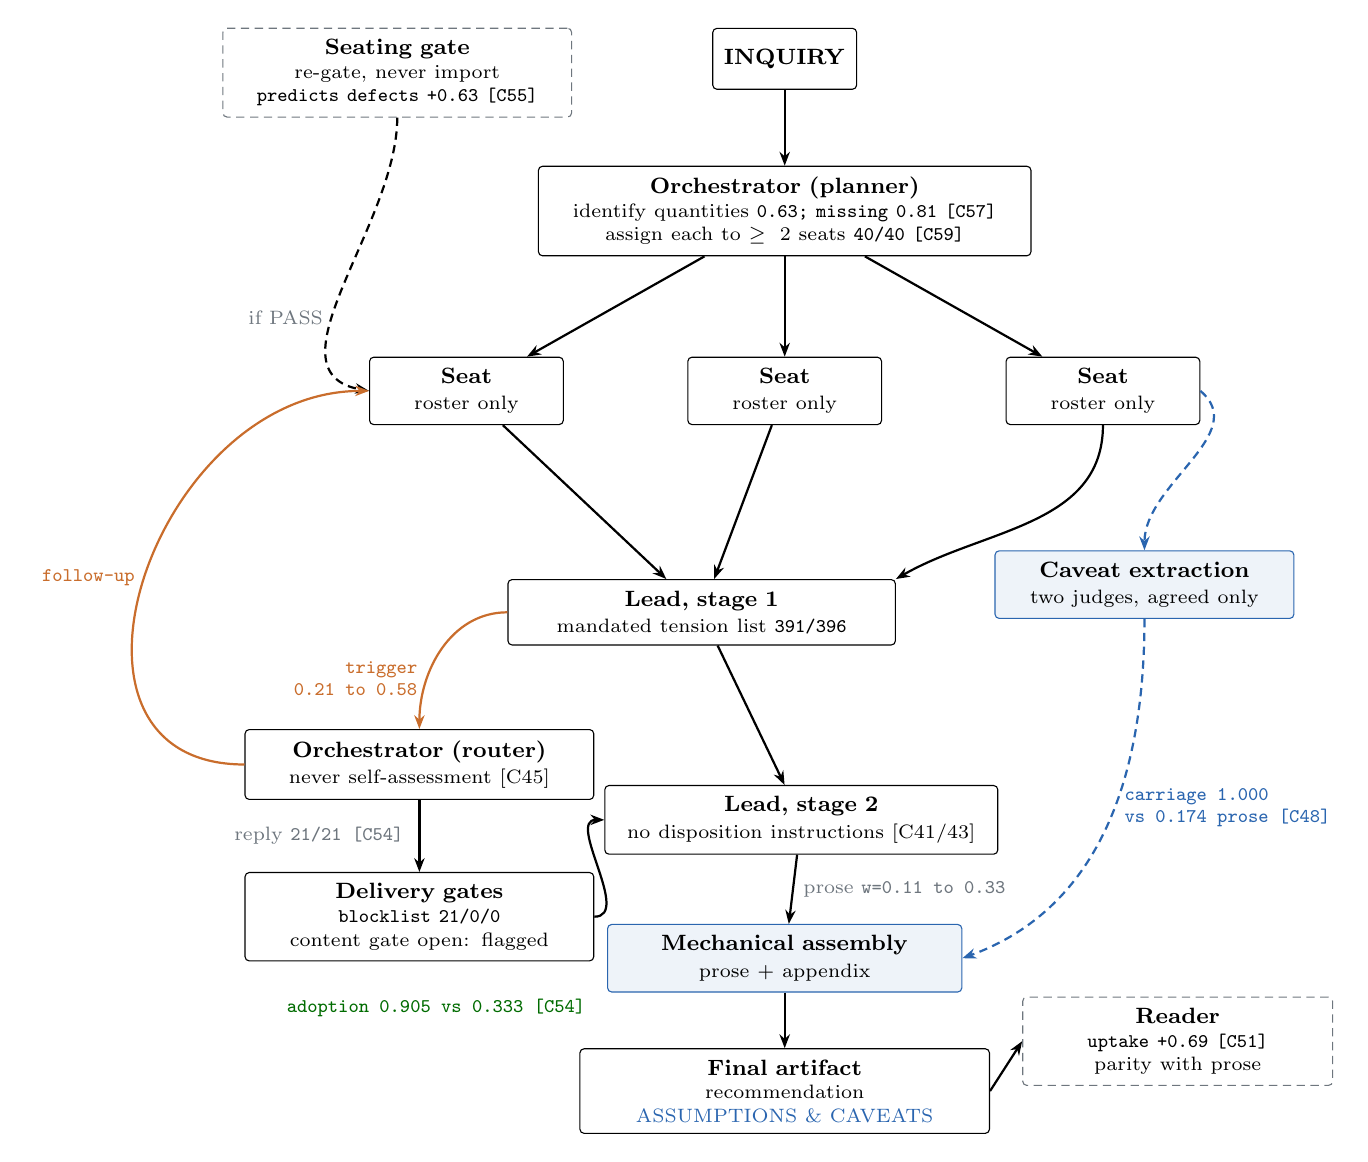
\begin{tikzpicture}[x=1pt,y=1pt,font=\footnotesize,
  box/.style={draw,rounded corners=1.5pt,align=center,inner sep=4pt,minimum height=22pt},
  gate/.style={box,densely dashed,draw=inkmut},
  frt/.style={box,draw=accent,fill=accent!8},
  ed/.style={-{Stealth[length=5pt]},thick},
  edf/.style={-{Stealth[length=5pt]},thick,accent,densely dashed},
  edl/.style={-{Stealth[length=5pt]},thick,corrupt},
  n/.style={font=\scriptsize\ttfamily,text=accent},
  ng/.style={font=\scriptsize\ttfamily,text=black!30!green!60!black},
  nr/.style={font=\scriptsize\ttfamily,text=corrupt},
  s/.style={font=\scriptsize,text=inkmut}]
\node[box] (q) at (170,395) {\textbf{INQUIRY}};
\node[gate,text width=118pt] (sg) at (30,390)
  {\textbf{Seating gate}\\[-1pt]{\scriptsize re-gate, never import}\\[-1pt]
   {\scriptsize\ttfamily predicts defects +0.63 [C55]}};
\node[box,text width=170pt] (pl) at (170,340)
  {\textbf{Orchestrator (planner)}\\[-1pt]
   {\scriptsize identify quantities \ttfamily 0.63; missing 0.81 [C57]}\\[-1pt]
   {\scriptsize assign each to $\ge2$ seats \ttfamily 40/40 [C59]}};
\node[box,text width=62pt] (s1) at (55,275) {\textbf{Seat}\\{\scriptsize roster only}};
\node[box,text width=62pt] (s2) at (170,275) {\textbf{Seat}\\{\scriptsize roster only}};
\node[box,text width=62pt] (s3) at (285,275) {\textbf{Seat}\\{\scriptsize roster only}};
\node[frt,text width=100pt] (cv) at (300,205)
  {\textbf{Caveat extraction}\\{\scriptsize two judges, agreed only}};
\node[box,text width=132pt] (l1) at (140,195)
  {\textbf{Lead, stage 1}\\{\scriptsize mandated tension list \ttfamily 391/396}};
\node[box,text width=118pt] (rt) at (38,140)
  {\textbf{Orchestrator (router)}\\{\scriptsize never self-assessment [C45]}};
\node[box,text width=118pt] (gt) at (38,85)
  {\textbf{Delivery gates}\\[-1pt]
   {\scriptsize\ttfamily blocklist 21/0/0}\\[-1pt]
   {\scriptsize content gate open: flagged}};
\node[box,text width=134pt] (l2) at (176,120)
  {\textbf{Lead, stage 2}\\{\scriptsize no disposition instructions [C41/43]}};
\node[frt,text width=120pt] (asm) at (170,70)
  {\textbf{Mechanical assembly}\\{\scriptsize prose + appendix}};
\node[box,text width=140pt] (fin) at (170,22)
  {\textbf{Final artifact}\\[-1pt]{\scriptsize recommendation}\\[-1pt]
   {\color{accent}\scriptsize ASSUMPTIONS \& CAVEATS}};
\node[gate,text width=104pt] (rd) at (312,40)
  {\textbf{Reader}\\[-1pt]{\scriptsize\ttfamily uptake +0.69 [C51]}\\[-1pt]
   {\scriptsize parity with prose}};
\draw[ed] (q) -- (pl);
\draw[ed,densely dashed] (sg.south) to[out=-90,in=170] node[s,left,pos=.6]{if PASS} (s1.west);
\draw[ed] (pl) -- (s1); \draw[ed] (pl) -- (s2); \draw[ed] (pl) -- (s3);
\draw[ed] (s1) -- (l1); \draw[ed] (s2) -- (l1);
\draw[ed] (s3.south) to[out=-90,in=30] (l1.north east);
\draw[edf] (s3.east) to[out=-40,in=90] (cv.north);
\draw[edf] (cv.south) to[out=-90,in=20]
  node[n,right,pos=.45,align=left]{carriage 1.000\\vs 0.174 prose [C48]} (asm.east);
\draw[edl] (l1.west) to[out=180,in=90]
  node[nr,left,pos=.7,align=right]{trigger\\0.21 to 0.58} (rt.north);
\draw[edl] (rt.west) to[out=180,in=180,looseness=1.4]
  node[nr,left,pos=.5,align=right]{follow-up} (s1.west);
\draw[ed] (rt) -- node[s,left=2pt]{reply \ttfamily 21/21 [C54]} (gt);
\draw[ed] (gt.east) to[out=0,in=180] (l2.west);
\node[ng] at (44,52) {adoption 0.905 vs 0.333 [C54]};
\draw[ed] (l1) -- (l2);
\draw[ed] (l2) -- node[s,right]{prose \ttfamily w=0.11 to 0.33} (asm);
\draw[ed] (asm) -- (fin);
\draw[ed] (fin.east) -- (rd.west);
\end{tikzpicture}
\caption{The assembled harness on one inquiry, with every edge labeled
by its registered measurement. Dashed blue: the out-of-band channel
for epistemic qualification, which the writer never sees. Orange: the
orchestrator-routed re-consultation loop, bounded by its measured
trigger rate. Seats are interchangeable by industry; chairs are earned
by the gate, never by category label. Engineered overlap between seats
is where the error immunity resides: corrupted-value adoption falls
from $0.90$ to $0.45$ [C47], and the clean co-source is used
end-to-end at $+0.43$ [C59].}
\label{fig:arch}
\end{figure}

\subsection{Design principles}

The harness follows four principles, each licensed by a verdict.

\begin{enumerate}
\item \textbf{Engineer coverage rather than assume verification.} The
source-selector result establishes that protection against error is a
function of which sources exist, not of any checking the lead performs.
\item \textbf{Carry epistemic content outside the writer.} The
transport bound establishes that prose loses two thirds to nine tenths
of the qualification supplied to it, and the preference result
establishes that in-prose marking is penalized.
\item \textbf{Trigger from artifacts, not self-assessment.} The
consultation results establish that models act correctly when
dispatched but do not reliably recognize the need to be dispatched.
\item \textbf{Retain nothing on rationale alone.} Every component
carries the registered verdict that licenses it, including verdicts
that demoted the original design rationale.
\end{enumerate}

\subsection{Components}

\paragraph{Seating is empirical, never categorical.} Because
signatures are per-model, no seat is chaired for its category label. A
candidate passes a measured gate consisting of a degeneracy screen (at
least $800$ visible characters on screen items; one archive fine-tune
produced $12/12$ degenerate probe runs), a tuned-minus-own-base
signature probe, and a format smoke test at production token budgets. A
generalist under a role prompt is a legitimate seat if it passes; most
experiments in the program ran on exactly that configuration.

\paragraph{Isolation, on cost grounds only.} Seats receive their task
and a one-line roster. Sibling outputs are not forwarded. The original
contamination rationale for this rule was withdrawn
(Section~\ref{sec:retests}); the rule survives because sibling context
costs approximately $10$k input characters and $14\%$ longer outputs
per seat while purchasing no measured change in lane discipline.

\paragraph{Redundancy is engineered.} The orchestrator identifies
load-bearing quantities in the decomposition and assigns each to at
least two seats. This is where the council's error immunity resides; it
does not exist by default.

\paragraph{Triggers come from mandated artifacts.} The lead runs in two
stages: a mandated tension list first ($391/396$ archived runs produce
one when required), then synthesis. The orchestrator, never any model's
disposition or self-assessment, parses the list and dispatches
follow-ups. A reply that adds nothing beyond the seat's first
contribution is flagged rather than delivered silently (a ritual-effect
risk observed at $d\approx0.22$, below the power to confirm, is treated
as live).

\paragraph{Epistemic qualification travels out-of-band.} Caveats,
assumptions, and confidence never route through the writer. Seats emit
them as structured fields, and the harness carries them mechanically to
an appendix of the final artifact. The writer receives no disposition
instructions at all: the evidence indicates that such instructions
purchase nothing and that their surface forms cost preference.

\paragraph{A Goodhart charter.} Trigger rates, hedge counts, compliance
shares, transport slopes, and preference scores on epistemic content
are diagnostics and may never be optimization targets; the optimizable
signal must live outside the pipeline's own text. Each entry on the
forbidden list cites the experiment that showed what optimizing it
would manufacture.

\section{Prospective Re-tests of the Harness}
\label{sec:retests}

Design rules distilled from findings can still be wrong, because
post-hoc patterns calcify. Each load-bearing rule therefore received its
own registered experiment, with kill conditions stated in advance. The
verdicts follow.

\subsection{The seating gate predicts pipeline defects (survived)}

Ten local candidates were gated on the frozen degeneracy screen, using
two screen items disjoint from the pipeline case set, with verdicts
committed to the repository before any pipeline run. Every candidate
was then seated on the pipeline cases. Strict rank separation held:
both gate-fail candidates defected in the pipeline ($0.333$ and $0.944$
of contributions) while all eight gate-pass candidates ran at $0.000$
to $0.056$; the pooled contrast is $+0.632$ \ci{+0.549}{+0.722}. Two
refinements followed. First, gate verdicts age: one model that passed
the archive-era screen failed the fresh re-gate and then defected
in-pipeline at $0.333$, so seating must re-gate rather than import a
stored verdict. Second, format compliance is a separate axis that does
not predict seat defects; the legal fine-tune failed the format smoke
test $0/4$ yet seated defect-free, so that component's proper target is
verdict-emitting roles.

\subsection{The planner chain works, measured link by link (survived,
with bounds)}

The redundancy planner was the one component that had never been
exercised: every prior redundancy result used human-planted
assignments. Three experiments closed the gap. \emph{Identification:}
the orchestrator recalls load-bearing quantities at $0.633$
\ci{0.506}{0.758} against analyst-authored labels (a thirty-fold
specificity separation over a mismatched-case control), unchanged by
seeing the specialists' contributions, so it runs at decomposition
time. Its best class is the right one: \emph{missing} quantities
(unmeasured rates, untracked inputs) are identified at $0.813$ against
$0.531$ for stated figures. \emph{Assignment and use, fully live:}
given the identified quantity, the planner writes it into at least two
sub-questions in $40/40$ plans; live seats convey briefed values at
$0.85$ to $0.95$; and the writer uses the clean co-source end-to-end
($+0.425$ \ci{+0.325}{+0.525} clean adoption against the planted
$+0.500$). A halted first attempt produced a channel finding: privately
briefed facts convey only into task-relevant assignments ($2/8$ when
orthogonal against $21/21$ when pointed), a constraint the corrected
planner input satisfies by construction. Expected end-to-end protection
is therefore the product of identification coverage (approximately
$0.63$) and the selection effect.

\subsection{The content gate failed (recorded as not deployable)}

The rule that follow-up replies adding nothing should be dropped failed
two registered attempts on complementary halves. A two-judge semantic
gate passes vacuous fillers ($3/6$ dropped), and an extract-then-verify
gate that fixes vacuity ($6/6$) rejects $52\%$ of genuine live replies.
Under the frozen commitment there is no third attempt without
purpose-built labeled data; the interim posture is flagged delivery,
never silent gating. The fabrication blocklist gate, by contrast, is
deployable: $21$ true hits, $0$ false positives, and $0$ misses over the
$141$-reply archive, seeded only from committed classifications. The
failed gate is reported beside the deployed one because refusing that
asymmetry is the method.

\subsection{Redundancy is causal (survived)}

A single factor, assigning the contested quantity to a second seat,
halved corrupted-value adoption from $0.900$ to $0.450$
(\ci{+0.200}{+0.725}), with the clean value actually adopted (from
$0.000$ to $0.500$). This is selection rather than dilution. The bare
arm's $0.900$ also stands as the sharpest no-verification measurement
on record. Protection is bimodal across items; two candidate boundary
mechanisms were then registered and rejected (prior plausibility at
$0.544$; the elicited ownership map at exactly $0.500$ prospective
against $0.895$ descriptive, with a minimum detectable difference of
$0.68$, the confirmation experiment performing its anti-calcification
function). The boundary is open and stated as such.

\begin{figure}[t]
\centering
\begin{minipage}{0.44\textwidth}
\centering
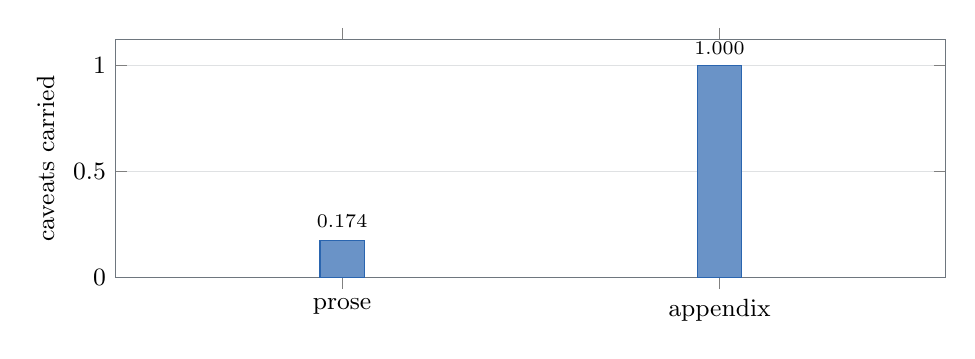
\begin{tikzpicture}
\begin{axis}[width=\textwidth,height=4.6cm,ybar,bar width=16pt,
  ymin=0,ymax=1.12,xtick={1,2},xticklabels={prose,appendix},
  ylabel={caveats carried},xmin=0.4,xmax=2.6,
  tick label style={font=\small},ylabel style={font=\small},
  axis line style={inkmut},ymajorgrids,grid style={inkmut!22}]
\addplot+[fill=accent!70,draw=accent] coordinates {(1,0.174) (2,1.000)};
\node[font=\scriptsize,anchor=south] at (axis cs:1,0.19) {0.174};
\node[font=\scriptsize,anchor=south] at (axis cs:2,1.005) {1.000};
\end{axis}
\end{tikzpicture}
\end{minipage}\hfill
\begin{minipage}{0.53\textwidth}
\centering
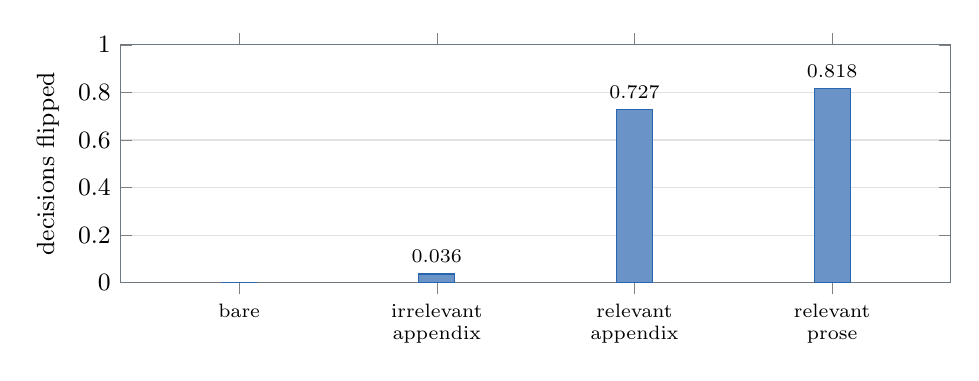
\begin{tikzpicture}
\begin{axis}[width=\textwidth,height=4.6cm,ybar,bar width=13pt,
  ymin=0,ymax=1.0,xtick={1,2,3,4},
  xticklabels={bare,{irrelevant\\appendix},{relevant\\appendix},
  {relevant\\prose}},xticklabel style={font=\scriptsize,align=center},
  ylabel={decisions flipped},xmin=0.4,xmax=4.6,
  tick label style={font=\small},ylabel style={font=\small},
  axis line style={inkmut},ymajorgrids,grid style={inkmut!22}]
\addplot+[fill=accent!70,draw=accent] coordinates
  {(1,0.000) (2,0.036) (3,0.727) (4,0.818)};
\node[font=\scriptsize,anchor=south] at (axis cs:2,0.045) {0.036};
\node[font=\scriptsize,anchor=south] at (axis cs:3,0.732) {0.727};
\node[font=\scriptsize,anchor=south] at (axis cs:4,0.823) {0.818};
\end{axis}
\end{tikzpicture}
\end{minipage}
\caption{The out-of-band channel, tested on both halves. \emph{Left}:
caveat carriage through writer prose against the mechanically assembled
appendix (zero-generation design). \emph{Right}: registered two-token
reader decisions flipped by a planted decision-relevant caveat, by
delivery arm; the irrelevant-appendix control shows that the effect is
content rather than appendix presence. Uptake is $+0.691$
\ci{+0.455}{+0.891}; parity with prose is $+0.091$
\ci{-0.036}{+0.218}.}
\label{fig:freight}
\end{figure}

\subsection{Out-of-band qualification carries and is used (survived)}

\emph{Carriage:} the appendix delivers $1.000$ of both-judge caveat
sentences against $0.174$ surviving prose, with no detected preference
penalty ($0.510$ \ci{0.267}{0.754}; not evaluable at power, reported
as bounded). \emph{Uptake:} appendix-delivered caveats flip a reader's
registered decision at $0.727$ against $0.036$ for the identical block
carrying an irrelevant caveat, with direction-balanced items so that
caution cannot masquerade as uptake, at parity with in-prose placement
(Figure~\ref{fig:freight}). The channel that preference judging cannot
see is not an exhibit; it changes decisions.

\subsection{The live loop closes (survived, with one halt)}

A first live-specialist experiment buried the deciding fact in the
specialist's own round-one text and halted at its registered pilot
gate: the trigger named the tension at only $0.208$ with the fact
visible in the pile. The redesign supplied the fact as the specialist's
private working notes, knowledge held but never written, and restored
the original round-one bytes. The live specialist conveyed the fact
$21/21$ times when dispatched; the lead adopted at $0.905$ against
$0.333$ archived control ($+0.571$ \ci{+0.139}{+0.912}), within
$-0.095$ \ci{-0.227}{0.000} of the scripted ceiling. One new risk is on
record: $4/21$ live replies embellished the correctly conveyed fact
with fabricated authority (invented case law, invented regulatory
rulings) and were adopted regardless. Content gates screen absence, not
invention; the fabrication rate was subsequently bounded
(Section~\ref{sec:economics}).

\subsection{Isolation lost its warrant (demoted)}

The registered one-factor test made byte-fixed sibling contributions
visible under production prompts. Off-domain framework density moved
$-0.009$ \ci{-0.048}{+0.028} against a pre-registered minimum
detectable difference of $+0.05$ to $+0.08$ computed from the archive,
an informative null, with in-domain density unchanged. The
contamination rationale is withdrawn; the rule stands on cost. A
registered secondary measure pointed in the opposite direction: seats
shown their siblings' coverage used slightly fewer off-domain terms of
their own ($-0.033$ \ci{-0.053}{-0.013}). This is recorded as a
candidate mechanism, not claimed.

\subsection{The ownership rule failed confirmation (rejected)}

A stable, near-unanimous elicited map of which seat ``owns'' each
quantity, exactly the kind of pattern a framework would ship as a
routing table, predicted arbitration at chance on fresh items. This
rejection is reported with the survivals because it is the argument:
the difference between an evidence-bound harness and a prompt stack is
that the harness can lose these arguments on the record, component by
component.

\subsection{The assembled bundle shows no detectable preference cost
(survived)}

With every component separately verdicted, the remaining deployment
question was head-to-head: the assembled harness's artifact against the
original architecture's, on the validated order-debiased two-family
protocol ($108$ pairs). The result is no evaluable difference:
primary-judge share $0.562$ \ci{0.375}{0.765}, replication $0.333$
\ci{0.083}{0.562}, both spanning $0.5$, with large effects excluded in
both directions. The harness's preference standing is inherited from
aggregation itself, which both bundles share; its differentiators were
never preference plays, and shipping them (five caveats per artifact, a
follow-up round, restructured seats) costs nothing detectable. The
appendix's within-pair attribution is mildly positive ($+0.073$ toward
the harness). One descriptive statistic from the same experiment
reframes the loop's economics: on organic inquiries the orchestrator
dispatched a follow-up on $46/54$ pipelines ($0.85$). Real disagreement
between seats is abundant, against the $0.21$ to $0.58$ trigger range
measured on planted tensions.

\section{Operating Economics and Open Risks}
\label{sec:economics}

\paragraph{The trigger bounds coverage, less than anticipated.}
Everything downstream of the trigger is measured and works. On planted
tensions the trigger fires at only $0.208$ to $0.583$ by batch, and it
is deliberately not an optimization target, because raising it blindly
manufactures the ritual condition that the loop's own control arm
exposed. The bundle comparison's telemetry reframes the economics: on
organic inquiries, where seats genuinely disagree, dispatch fired on
$0.85$ of pipelines. The scarcity that bounded the experimental cells
largely dissolves on natural problems; planted-tension rates are the
floor rather than the forecast.

\paragraph{Open risks.} Per-item protection is bimodal with the
boundary mechanism unknown (two candidates rejected). Live-reply
fabrication is bounded by a registered follow-up experiment:
reply-level $0.100$ \ci{0.047}{0.201} with the deciding fact in hand
and $0.150$ \ci{0.081}{0.261} without it, concentrated entirely on one
trigger topic ($15/20$ there, $0/100$ elsewhere) and name-stable, with
the same two invented decisions recurring across independent samples,
which licenses a blocklist delivery filter. The seat never admits the
gap ($0/20$ sampled), the backfill mechanism is directionally positive
but not evaluable at six clusters, and the bound covers adversarial
case citations only, a floor rather than a ceiling on confabulation.
The preference cost of the appendix is bounded but not evaluable at
current power. The council's accuracy question is resolved as
untestable for lack of headroom: two registered batteries (multi-step
computation; rule-path selection) placed the direct writer at ceiling
($0.977$, $0.983$) under baseline-only difficulty screens, so no
well-specified known-answer battery can measure a council difference at
this scale. This is the strongest available statement of the design
rule that a council is not an accuracy device. None of these risks is
hidden in the architecture document; each is attached to the component
it concerns.

\paragraph{Running the harness replicates the science.} The harness's
telemetry doubles as a replication battery. Every deployment yields
transport estimates, trigger telemetry, phrase-swap slots for proposed
instructions, and preference-versus-verified divergence wherever ground
truth exists, each with its attainability gate. A faithful deployment
is also, at near-zero marginal cost, the external validation that the
program's scope caveats call for.

\section{Limitations}
\label{sec:limits}

The scope is 7 to 20B local models, advisory-domain English, and one
primary writer family, with cross-family replications where stated.
Cluster ceilings of 6 to 18 items bind every harness experiment; the
live-loop comparison uses archived arms under a registered fresh-batch
check; the uptake verdict covers 11 of 18 authored items after a
registered floor gate; and trigger rates are batch-variable and quoted
only as a range. The harness's gains are preference, immunity, and
resolution, not accuracy, which two registered batteries resolved as
untestable at this scale: the direct writer ceilings at $0.977$ to
$0.983$ on well-specified items, so no headroom exists (under-specified
or adversarial constructions would pose a different question). Verdicts
inherit their experiments' scope and should not be generalized past it;
the architecture document states, for every component, exactly which
registered experiment licenses it.

\section{Conclusion}
\label{sec:conclusion}

A council-of-experts pipeline was built on premises that nearly all
failed registered tests. The failures were informative: each localized
a mechanism, and the mechanisms composed into a harness whose every
component is licensed by a specific verdict. Prospective re-tests
confirmed the load-bearing components with causal or predictive effect
sizes, demoted one design rationale, rejected one candidate rule,
recorded one gate as not deployable, and found that the assembled
bundle ships its machinery at no detectable preference cost. The
resulting architecture is smaller than the one designed and better
supported than the one assumed. The practice proposed for adoption is
the acquisition path itself: retaining only what survives registered
attempts to falsify it, and reporting the demotions in place beside the
survivals.

\section*{Reproducibility Statement}

The complete pre-registration ledger (52 registration blocks at this
writing), every deviation and verdict including the two halts, the
architecture document, the measurement kit (\texttt{gst}), the frozen
dictation registry, and all item files are in the project repository.
Registrations are committed before first runs, so temporal ordering is
verifiable from version history.

\begin{thebibliography}{9}
\bibitem{wang2024moa} J.~Wang, J.~Wang, B.~Athiwaratkun, C.~Zhang,
J.~Zou. Mixture-of-Agents enhances large language model capabilities.
\emph{arXiv:2406.04692}, 2024.
\bibitem{bobo2026audit} S.~Bobo. Instructions buy the phrase; the
phrase costs preference: an epistemic audit of LLM aggregation
pipelines at auditable scale. Companion draft, 2026.
\bibitem{li2025selfmoa} W.~Li et al. Rethinking Mixture-of-Agents: is
mixing different large language models beneficial?
\emph{arXiv:2502.00674}, 2025.
\bibitem{zheng2023judging} L.~Zheng et al. Judging LLM-as-a-judge with
MT-Bench and Chatbot Arena. \emph{NeurIPS Datasets and Benchmarks},
2023.
\bibitem{singhal2023length} P.~Singhal et al. A long way to go:
investigating length correlations in RLHF. \emph{arXiv:2310.03716},
2023.
\bibitem{sharma2023sycophancy} M.~Sharma et al. Towards understanding
sycophancy in language models. \emph{arXiv:2310.13548}, 2023.
\bibitem{wang2024rebuttal} Q.~Wang et al. Rethinking the bounds of LLM
reasoning: are multi-agent discussions the key?
\emph{arXiv:2402.18272}, 2024.
\end{thebibliography}

\end{document}
